\documentclass[man,noapacite]{apa2} 

\usepackage{apacite2}
\usepackage{amssymb}
\usepackage{graphicx}

\title{Using Tablets to Collect Data from Young Children} 

\author{Michael C. Frank, Elise Sugarman, Alexandra Horowitz, \\ Molly L. Lewis, \& Daniel Yurovsky} 

\affiliation{Department of Psychology, Stanford University}

\abstract{Mobile, touch-screen devices are increasingly ubiquitous in children's lives. The extensive use of such devices provides both a challenge and an opportunity for developmental psychologists. While more research is needed to understand the nature and consequences of young children's interaction with such devices, they nevertheless present an exciting opportunity for data collection. We describe a simple method for creating cross-platform, interactive tablet experiments using open web-based resources. We illustrate this method by collecting data from children 1--5 years old in a simple word-recognition paradigm and show that it yields reliable reaction time and accuracy data from young children. Tablets should be considered by researchers as a viable method for collecting low-cost, well-controlled developmental data.}

\shorttitle{Tablet-based Data Collection} 
\rightheader{TABLET-BASED DATA COLLECTION}

\acknowledgements{We gratefully acknowledge the laboratory of Anne Fernald for sharing their stimuli and the families and staff at San Jose Children's Discovery Museum. An earlier version of this material was previously presented in a blogpost \cite{frankblogpost}. Thanks to Janelle Klaas, Andrew Weaver, and Sarah James for assistance in data collection. Please address all correspondence to Michael C. Frank, Department of Psychology, Jordan Hall (Bldg. 420), 450 Serra Mall, Stanford, CA 94305. Phone: (650) 724-4003. E-mail: \texttt{mcfrank@stanford.edu}}

\begin{document}

\maketitle

%\setlength{\textfloatsep}{0.02cm}

\section{Introduction}

Since Apple debuted the iPad in 2010, the ubiquity of personal tablets---interactive, touchscreen-based computing devices, typically larger than a phone but smaller than a laptop---has skyrocketed. By 2013, an estimated 75\% of families with young children in the United States owned a mobile device, with 40\% of households owning tablets \cite<20\% of lower-income families and 63\% of higher-income families;>{rideout2014}. At present, tablets are estimated to constitute 19\% of children's overall screen time from ages 0--8. This explosion in popularity has created a surge of interest in both the consequences of tablet use for children and the potential for using these devices as scientific tools. 

Nevertheless, there are significant challenges involved in using tablets for research. These include the difficulty and potential costliness of developing custom applications (``apps'') for individual experiments, technical problems with app distribution and cross-device compatibility, and the lack of data confirming the validity of the tablet data collection method. Perhaps for these reasons, there is currently a paucity of published articles that use tablets to collect developmental data. 

The goal of the current article is to address these challenges. We begin by briefly reviewing research on the use of tablets in children. We then describe a method for using standard, freely-available web-development tools to create tablet-based experiments. Although this method requires some programming experience, it is significantly easier than developing tablet-native applications and has relatively few drawbacks from the research perspective. We next show how this method can be used to implement a simple word-recognition experiment. Our data suggest that the tablet platform is an engaging method for data collection that yields reliable accuracy and reaction time from children two years old and perhaps even younger. 

\section{Children's Tablet Use}

Children's ability to learn from entertainment technologies is contested. A number of influential studies suggest that children learn less from videos than they do from live demonstrations, a phenomenon known as the video deficit effect \cite<e.g.>{anderson2005,deloache2010,kuhl2003}.A survey of parent reports of television-viewing and children's vocabulary under age 2 found that infants who spent more time viewing infant-directed programs (``baby media,'' such as the Baby Einstein series), had lower vocabulary (\citeNP{zimmerman2007}; but see \citeNP{ferguson2014} for a recent reevaluation of these data). These findings influenced the American Academy of Pediatrics (AAP) to uphold a policy recommending no ``screen time'' for children under age 2 \cite{brown2011}.

Although screen media may not offer as rich a pedagogical experience as live interaction, the experiences offered by touch-screen devices may be distinct from passive viewing of television and computer screens. \citeA{christakis2014} notes that the AAP's published media recommendation of no screen time was made before the release of tablet devices, and suggests that the policy should be revised to distinguish and accommodate some time with touch-screens. He proposes that tablets can offer a number of potential benefits that many traditional toys do not. Specifically, tablets are reactive (responding contingently to the child’s actions), interactive (eliciting responses from the child based on his or her actions), tailorable (modifiable according to age or preference), progressive (can increase in difficulty or complexity with experience), highly portable, and able to promote joint attention (a child and caregiver can interact with the program together). 
% Touch screens offer an interactive experience with feedback contingent on the child's touch; these devices have a range of features that can be individualized to a child's age and performance. 

While screens are not recommended as replacements for live interactions, interactive technologies may pose a number of benefits over other passively-viewed screen alternatives. Some work suggests that practice with interactive games may benefit attention and motor control \cite{bavelier2010}, and more generally screen time with tablets can promote independence, opportunities for physical closeness, and feelings of fun and accomplishment \citeA{rvachew2013}. The contingent feedback and individualization offered by mobile devices may thus make them a better medium for learning and engagement than traditional view-only screens. Such benefits may also make them valuable tools for research and evaluation.

In addition, young children do demonstrate some learning from interactive screen content, suggesting that ``video deficit'' effects may be limited to---or at least strongest in---passive viewing of pre-recorded material. In one study, \citeA{roseberry2014} found that 24- to 30-month-olds successfully learned a novel verb from a live interaction via video chat, while a yoked group who saw the same input with non-contingent presentation failed to learn.
% They taught 24- to 30-month-olds novel verbs in one of three conditions: in-person demonstration, video chat demonstration, or a yoked video demonstration (recorded from a different child, therefore not socially-contingent to the participant). They found that toddlers were able to learn the new verbs above chance and equally well for both of the socially-contingent conditions (in-person and video chat demonstrations), but were only at chance in the control condition. Even despite challenges from in-person information (e.g. skewed gaze cues due to the position of the camera), the contingent feedback appears to drive children’s ability to learn through live video interactions.
Young children also show some evidence of transferring learning between screens and physical objects. \citeA{zack2009} examined 15-month-olds' ability to transfer knowledge learned via a touch-screen or physical toy to another example either in the same presentation modality or across modalities. Children were most successful when toys were presented in the same modality, but children in the cross-modality conditions performed better than a no-demonstration baseline. Even before age 2, children thus show evidence of comprehending actions and goals presented on touch-screen devices and can transfer this knowledge between physical and 2-dimensional presentations.

One concern with children's performance is the accuracy of their motor control. \citeA{couse2010} found that young children could quickly learn to provide precise motor input on tablets with minimal training using a stylus pen. They had teachers rate the quality and complexity of 3- to 6-year-old's self-portraits created digitally on a tablet art program compared with their drawing using traditional writing tools on paper. Children were highly engaged with tablet program, their drawings were rated as typical or exceeding their typical quality of drawing, and three quarters of children on the tablet task exhibited no to little frustration during the task despite a number of technical challenges. Additionally, although researchers were prepared to give children up to four warm-up sessions using a stylus pen on tablet computer, most children advanced after a single warm-up phase. Altogether, these studies suggest that preschoolers and kindergarteners are highly motivated and competent at interacting with touch-screen tablets. 

And although children show interest and remarkable capabilities to use touch-screens even before they learn to talk, some affordances of mobile tablets are easier to master from young ages than others. \citeA{aziz2014} tested 2- to 5-year-olds in Malaysia and the United Kingdom on their ability to perform the seven most common touch gestures of iPads: tap, drag/slide, free rotate, drag and drop, pinch, spread, and flick. By age 2, children mastered the tap and drag/slide gestures, and by age 3, they could reliably produce all by the spread gesture. By age 4, all children performed all of the gestures. In sum, designers of tablet materials for young children should consider appropriate content and gesture capabilities according to the target age.
% , and precision of touch input may be increased with tools such as fine-tipped stylus pens instead of finger touches.

\section{Collecting Developmental Data With Tablets}

\subsection{The value of tablet-based data collection}

Researchers working with young children have access to a wide variety of experimental paradigms, ranging from behavioral forced-choice to eye-tracking and looking-time based measures \cite{aslin2007,gredeback2009}. Nevertheless, each of these methods has its drawbacks: behavioral methods are flexible and easy to implement, but they can be subject to experimenter biases, and often require labor-intensive offline coding. In contrast, corneal-reflection eye-tracking methods are precise and unbiased, allowing tight experimental control, but can be expensive and are difficult to implement outside of tightly-controlled lab settings. In addition, they are typically limited in length as they tend to be non-interactive.

Tablet-based experimental paradigms can supplement both of these data collection modalities by allowing researchers to create engaging, interactive paradigms that are low cost but nevertheless offer some of the precision and experimental control of eye-tracking paradigms. In the sections below, we offer five reasons why tablets may be valuable tools for developmental research.

\subsubsection{Diverse measures} Tablets allow the collection of many different dependent variables, including forced-choice responding and gesture trajectories. We especially highlight the ability to measure reaction times using tablets. Reaction times provide a continuous, informative measure of cognitive process and have proven invaluable in both developmental \cite<e.g.>{fernald1998,marchman2008} and adult \cite<e.g.>{sternberg1969} studies. Behavioral paradigms that afford reaction time measurement for young children typically require time-consuming offline coding. In contrast, eye-tracking paradigms yield reaction times, but with the tradeoff that the paradigms typically have limited interactivity. 

\subsubsection{Engagement} Children across ages enjoy tablets and are highly motivated to explore new tablet-based tasks, allowing researchers to collect more data from individual children. As documented by  \citeA{couse2010} and many informal observations of infants' and young children's interest, the use of tablet-based devices may lead children to view tablet-based experiments as similar to engaging commercial apps. In addition, behavioral paradigms with young children often require a ``warm-up'' period so that the child is comfortable interacting with an unfamiliar experimenter; such a period can be shorter or absent to the extent that a tablet-based paradigm requires less face-to-face interaction. 

\subsubsection{Experimental control} Studies that involve interaction with an experimenter are the de-facto standard in cognitive development research, but such studies have as major drawbacks that it may be difficult or impossible to ensure that experimenters are blind to condition and hypothesis---often hypotheses are simple enough that even ``na\"ive'' research assistants can infer the experimental structure or the desired response. While there are methods for avoiding such issues, the possibility of eliminating experimenter bias via computerized stimulus presentation is an attractive method for situations where it is possible. And even when bias is not introduced, there are significant challenges in training a group of research assistants to implement an experimental protocol uniformly. Thus, tablet-based experiments can alleviate concerns about bias and uniformity of experimental presentation.

\subsubsection{Inclusion of special populations} Tablets can be a valuable tool for working with children who have learning or physical disabilities, including ASD and dystopia \cite<e.g.>{cardon2012, waddington2014, chai2014, bertucco2013}); 

\subsubsection{Scale} The low cost and high accessibility make it possible to distribute tablets to research assistants who can collect data in a wider variety of locations (though not without concern about environmental distractions). In addition, it is in principle possible that children could contribute data to experimental studies via experiments administered by their parents or caregivers.\footnote{For an example of this method, see \texttt{http://lookit.mit.edu}, a web-based platform for looking-time experiments that engages parents as experimental confederates.} It is this latter possibility that might be truly revolutionary in terms of the scope of data collection, though there are many challenges that such research would need to overcome.

Despite all of these advantages, there are significant technical issues related to app creation that have slowed the adoption of tablet-based methods in developmental research. Creating tablet-native apps (that can be accessed through an Android or iOS tablet's main menu) requires substantial programming expertise---and worse yet, this expertise is not transferrable across tablet platforms. Developing a native app for iOS requires programming in Objective-C using Apple's proprietary app development tools; in contrast, development for Android requires programming in a Java variant. Both languages have specific software development tools (SDKs) that allow programmers to tailor their apps for various devices. 

There are certainly cases where having a robust, native app might lead to better performance or adoption. An experiment that requires substantial media or animation, use of the tablet's camera, or large-scale data transfer is likely to perform better as a natively written app. Similarly, standardized experimental tools are more easily distributed and used via Google Play or the Apple App Store, the standard distribution methods for commercial software. But the cost of developing such apps is substantial: either an investigator must learn a special-purpose programming language, or a programmer must be employed. This latter option is more common, but costs can easily run in the tens of thousands of dollars; in this sort of scenario, making scientifically-useful changes to an app may be undesirable because of added costs. 

\subsection{A web-based method for developing tablet experiments}

In contrast to these costly, special-purpose methods, we describe an alternative method for prototyping and collecting data on tablets. The method relies on creating the experiment as a simple webpage and then showing this page in the tablet's web browser. This method still requires some programming experience, but much less; in addition, it draws on open-source, freely-available tools that are relatively easy to master. Experimental ``apps'' are easily shared, modified, and ported across platforms, leading to faster iteration and data collection. In addition, it offers the ability to collect control data with adult participants on Amazon Mechanical Turk \cite{paolacci2010,crump2013} with virtually no changes. Our method has three components:

\begin{enumerate}
\item A JavaScript/CSS/HTML web page, which is the core of the experiment, 
\item A server-side PHP script to collect data in tabular format, and
\item A tablet device running a kiosk application to present the experiment. 
\end{enumerate}

\noindent We discuss each below.\footnote{Our work has used the Apple iPad as the primary tablet platform and we provide details that are tailored for this platform. Nevertheless, and unlike other methods, our method is in principle portable to a wide range of mobile devices with only very minor modifications.}

\subsubsection{Web-based experiment}

The first component of our system is a web-based experiment created using HTML, JavaScript, and CSS. This combination is currently the most common set of tools for the creation of interactive websites. HTML (HyperText Markup Language) forms the framework for the static content shown on the website, while CSS (Cascading Style Sheets) gives a consistent set of formatting options. JavaScript then controls the interaction functionality of the website. In particular, we make use of a JavaScript library called jQuery (\texttt{http://jquery.com}) that allows HTML elements like images, layouts, text, and media to be dynamically added, subtracted, and rearranged as participants interact with the resulting page. 

It is beyond the scope of this article to provide an introduction to creating JavaScript-based web experiments, but there are a wealth of available resources on this topic. These resources include both psychology-specific tutorials and more general introductions to the general HTML/JavaScript/CSS model. A sample experiment (as well as the server side code) is provided in the version control repository for this paper (\texttt{http://github.com/langcog/tablet\textunderscore norming}). 

Hosting a web-based experiment requires server space, which is often provided by universities but can also be purchased from commercial providers. We find that the requirements on such a server are typically not high, so the costs involved are minimal.



 % there is a lot of good material out there, especially from the Gureckis Lab at NYU (e.g. this blog post). There are also many tools for learning how to make websites using the now standard combo of JavaScript, HTML, CSS, and jQuery. Note that putting up such an experiment will require some server space. We use the space provided by Stanford for our standard university web pages, but all that's required is somewhere to put your HTML, JS, and CSS files.

\subsubsection{Server-side data collection}

The second component of our system is a simple script that allows the experiment to save data in tabular format. Every time a participant completes the experiment, their data is sent to this script, written in a language called PHP (a simple scripting language that is often used for backend web development). The script simply appends data from the experiment to a tabular data file. The script can be hosted on any web-accessible server that has been configured to run executable files of this type. In practice, this will often be the same server that hosts the experiment itself, though it need not be. Data are then retrieved from this server periodically using SFTP (Secure File Transfer Protocol). 

\subsubsection{Tablet configuration}

The third component of our system is an internet-connected tablet. The requirement for internet connectivity is perhaps the most substantial drawback of our method, relative to native apps. The tablet must either have wireless access (e.g., from the testing location or a mobile hotspot device) or else the tablet itself must have cellular connectivity. Once the tablet has access to the web, the tablet's browser can simply be directed to the experiment website. 

A major challenge of presenting experiments in the tablet's web browser is to ensure that children cannot accidentally or intentionally navigate away from the experiment, exit the browser, or change perspective (e.g. by zooming). In practice, we use two tools for this purpose: the first is Guided Access, a mode on the iPad that disables the hardware buttons. The second is Mobile Kiosk, an app that further locks the iPad into a particular view of a webpage. The combination ensures that the tablet presents the experiment as intended. With both of these systems in place, the ``look'' of the experiment is extremely similar to a native app. 

\section{Norming Data}
 
To test the reliability and broad developmental applicability of our tablet method, we implemented a simple word-recognition paradigm, which we tested with a cross-sectional sample of children ages 1--5 from a local children's museum. The basis of our experiment was work on the developing speed and accuracy of word recognition by Anne Fernald and colleagues \cite{fernald1998,fernald2006,bion2013}. 

We designed a two-alternative forced choice paradigm that both tested children's recognition of familiar words and asked them to make so-called ``mutual exclusivity'' inferences---that a novel label refers to a novel word rather than a familiar competitor \cite{markman1988}. While the causes of this latter inference are still a source of theoretical disagreement \cite{markman2003,diesendruck2001,frank2009,bion2013}, it is nevertheless a highly replicable finding that we predicted woud show substantial developmental change across our sample.  We were thus interested in measuring developmental changes in both accuracy and reaction time, both in recognizing familiar words and in making inferences about novel words. 

\subsection{Methods}

\subsubsection{Participants} 

We recruited a sample of XYZ children ages 1--5 (our recruitment goal was 20 in each of four 1-year age group) from the floor of San Jose Children's Discovery Museum. An additional XYZ children were recruited for the following reasons: parent interference (XYZ), insufficient reported English exposure ($>75\%$, a standard cutoff in our studies with this population; XYZ), XYZ. 

\subsubsection{Stimuli}

Visual stimuli consisted of images of sixteen familiar and eight novel objects. All were presented as cropped images on a gray background with approximately the same resolution and detail.  Audio stimuli consisted of a carrier phrase (``Can you find [the target]?''), into which we spliced recordings of the target words. All recordings featured a female speaker and were created following the procedures described in \citeA{fernald2008}. We selected a variety of words from the MacArthur-Bates Communicative Development Inventory word list \cite{fenson1994,fenson2007}, choosing some words that we were certain nearly all children would be very familiar with (e.g., ``car,'' ``dog,'' ``bottle,'') and others that were intended to be slightly more challenging (e.g., ``monkey,'' ``shovel,'' ``lion''). Novel words were mono- and di-syllabic words that had been used in previous experiments of this type (e.g. ``pifo,'' ``dax,'' ``kreeb''). We further included four fillers to break up the experiment (e.g., a picture of a train with a sentence of audio describing it).

\subsubsection{Procedure}

We created a simple page to help children learn to tap appropriately on the iPad. To advance past this training page, they needed to tap a set of five dots in random locations; each dot transformed into an ``X'' when tapped. After the child tapped all the dots, the experimenter could either advance the app to the experiment or rerun the training if they felt the child could use more practice. 

Experimental stimuli were then presented in one of two pseudorandom lists, in which trials (which contained a pair of pictures) were counterbalanced for order, target side, and XYZ. The experiment had 28 trials in total (8 of each of three trial type plus four fillers). The three trial types were \emph{Familiar Word} trials, in which two familiar pictures were presented and children were asked to select the image that matched a familiar word; \emph{ME Control} trials, in which a familiar and a novel image were presented and children were asked to select the image that matched a familiar word; and \emph{ME Inference} trials, in which a familiar and a novel image were presented and children were asked to select the image that matched a novel word. 

\subsection{Results}

% \subsubsection{Task completion}

\begin{table}[t]
\centering
\caption{Proportion children finishing the study and average number of trials out of 28 completed for all children, by age group.\label{tab:completion}}

\begin{tabular}{rcc}
  \hline
Age group & Proportion finishing & Average number of trials \\ 
  \hline
1-year-olds & 0.45 & 22.6 \\ 
2-year-olds & 0.86 & 27.1 \\ 
3-year-olds & 1.00 & 28.0 \\ 
4-year-olds & 0.81 & 27.4 \\ 
   \hline
\end{tabular}
\end{table}

Children were enthusiastic about the experiment, even though it contained a substantial number of trials. One-year-olds varied in their ability to complete the study, with most completing half or two thirds but not the full 28 trials. In contrast, the other groups successfully completed the experiment at high rates. Completion rate and average number of trials completed are given in Table \ref{tab:completion}.

\begin{figure}[t] 
  \begin{center} 
    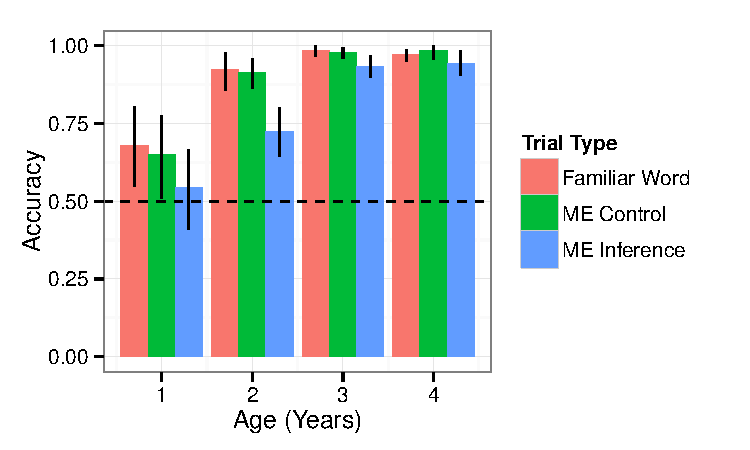
\includegraphics[width=5in]{figures/accuracy.pdf} 
    \caption{\label{fig:accuracy} Accuracy in our word recognition task, plotted by age group and trial type. Dashed line shows chance performance. Error bars show 95\% confidence intervals, computed by non-parametric bootstrap. }
  \end{center} 
\end{figure}

Accuracies for familiar word trials were above chance even for the one-year-old age group and rapidly approached ceiling performance in the two-year-olds (Figure \ref{fig:accuracy}). There were also no substantive differences in accuracy between Familiar Word and ME control trials. In contrast, ME Inference trials were substantially more difficult for children, with one-year-olds performing at chance, and two-year-olds showing a substantial decrement in performance for these trials. 

We fit a logistic mixed effects model with a maximal random effects structure \cite{barr2013} to the data. To make inferences about differences between age groups, we coded age group as a discrete factor.  We found significant main effects of age ($\beta = $, $p = $) and ME inference trials ($\beta = $, $p = $), but no effect of ME control trials ($\beta = $, $p = $). We additionally ...


\begin{figure}[t] 
  \begin{center} 
    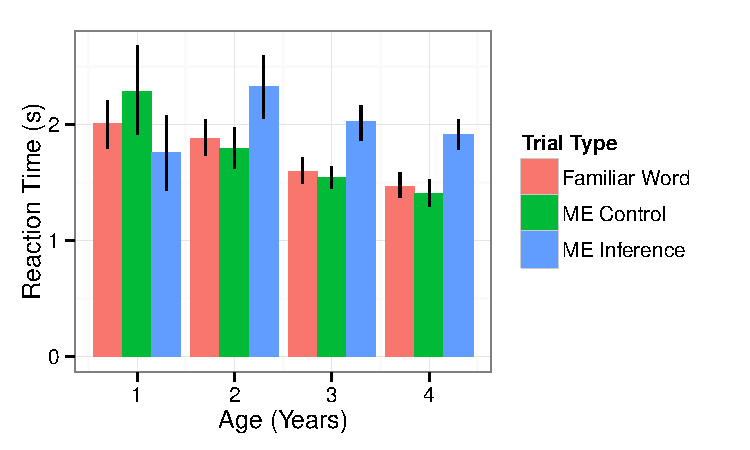
\includegraphics[width=5in]{figures/rt.pdf} 
    \caption{\label{fig:rt} Reaction times in our word recognition task, plotted by age group and trial type. Error bars show 95\% confidence intervals, computed by non-parametric bootstrap.}
  \end{center} 
\end{figure}

We next turned to reaction time data. Our reaction time data had a mean of XYZ but a median of only XYZ. This difference indicates a standard skewed distribution; in addition, the distribution contained a number of extreme outliers from trials where children asked for clarification, refused to choose, or simply became distracted. We removed outliers using a preset criterion of 2 standard deviations above or below the mean, computed in log space (lower threshold: XYZ ms, upper threshold: XYZ ms). This procedure removed XYZ\% of the data (around 1.XYZ trials of 28 per child). 

Reaction times showed both developmental and trial-by-trial effects. Older children were substantially faster at our task, and ME inference trials were slower than both Familiar Word and ME Control trials. Again, we did not observe large numerical differences between Familiar Word and ME Control trials.

We fit a linear mixed effects model to our reaction-time data. 

\begin{figure}[t] 
  \begin{center} 
    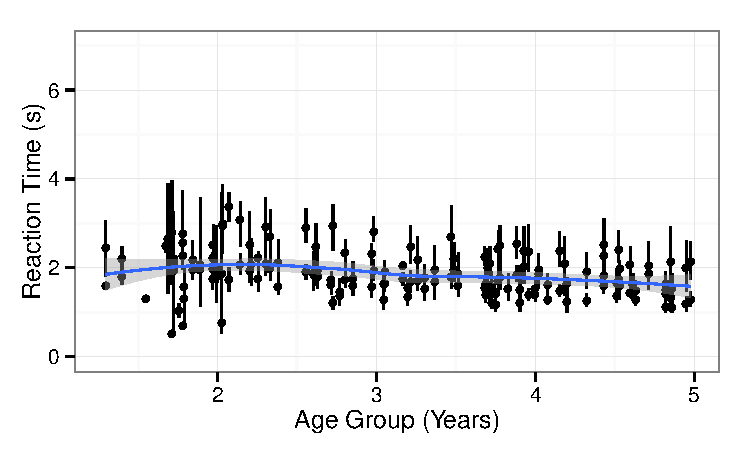
\includegraphics[width=5in]{figures/individuals.pdf} 
    \caption{\label{fig:rt2} Reaction times for familiar word recognition (both Familiar and ME control trials), plotted by age. Each dot represents an individual. Error bars show 95\% confidence intervals on individual RTs, computed by non-parametric bootstrap. The smoothing line is a loess non-parametric regression line with a 95\% confidence interval.}
  \end{center} 
\end{figure}

One primary concern for our study was the individual reliability of reaction time data. Group-level developmental differences such as those described above do not necessarily signal a measure with high reliability. We approach this question in several ways. First, we show individuals' reaction-time data plotted in Figure \ref{fig:rt2}, with confidence intervals for each. Confidence intervals are broad for the youngest children, but are relatively tight for the older children in our group. 

Next, we used the congruence between Familiar Word and ME Control trials to compute split-half reliability. FILL ME IN. 

\section{Conclusions} 

Mobile and tablet-based computers are quickly becoming a ubiquitous part of life---and of childhood. Children play with their parents' and their own devices, and such devices are used for education, reading, games, and video chat with friends and relatives. Many important developmental issues are raised by this ubiquity, and more research must be done to determine how, when, and what children can learn from different kinds of devices. Nevertheless, the opportunity posed by such devices for developmental psychologists is immense.

We presented a simple method for creating tablet ``apps'' that allows experimenters to create basic websites and use these websites to collect data on tablets. This method is substantially easier and more flexible than platform-native app development, which can be costly and time-consuming. In addition, it allows cross-platform compatibility and easy sharing for the resulting experiments. We showed in a simple word recognition experiment that this method yields reliable reaction time and accuracy data for children as young as two years of age. Data collection using tablets thus has the potential to supplement and perhaps even supplant many behavioral assessment methods currently in use. 

\newpage

\bibliographystyle{apacite}
\bibliography{tablet}

\end{document}
